\chapter{Introducción}
\label{ch:introduccion}
La sociedad en la que vivimos está cada vez más unida, y las fronteras se empiezan a disolver con el paso del tiempo. Citando a la Wikipedia, la globalización \cite{globalizacion} se define como \textit{``un proceso económico, tecnológico... que consiste en la creciente comunicación e interdependencia entre los distintos países del mundo... a través de una serie de transformaciones sociales, económicas y políticas que les dan un carácter global.''} Todavía quedan fronteras que a corto plazo no parece que vayan a desaparecer y lograr dicha interdependencia a escala mundial, pero no se puede negar este hecho.\\

Como podemos ver en el Apéndice 5.2 de \cite{globalreport}, la globalización supone un incremento económico, que cada año crece, de los paises que salen de sus fronteras para establecer relaciones con otros territorios a lo largo del globo. Pero la globalización no es solo un fenómeno económico, en él también se ven involucradas las \textit{nuevas tecnologías}.\\

Cuando salimos a la calle, vemos a muchas personas utilizando sus \textit{smartphones}, socializando, comunicándose con sus familiares y conociendo la actualidad internacional. Durante la última década, el uso de Internet se ha visto muy incrementado. Tal y como podemos ver en la imágen \ref{internetusageimagen} , en junio de 2017 se contabilizó que casi el 50\% de la población mundial hace uso de Internet, siendo este porcentaje de más del 80\% en países desarrollados.\\

\begin{figure}
    \centering
    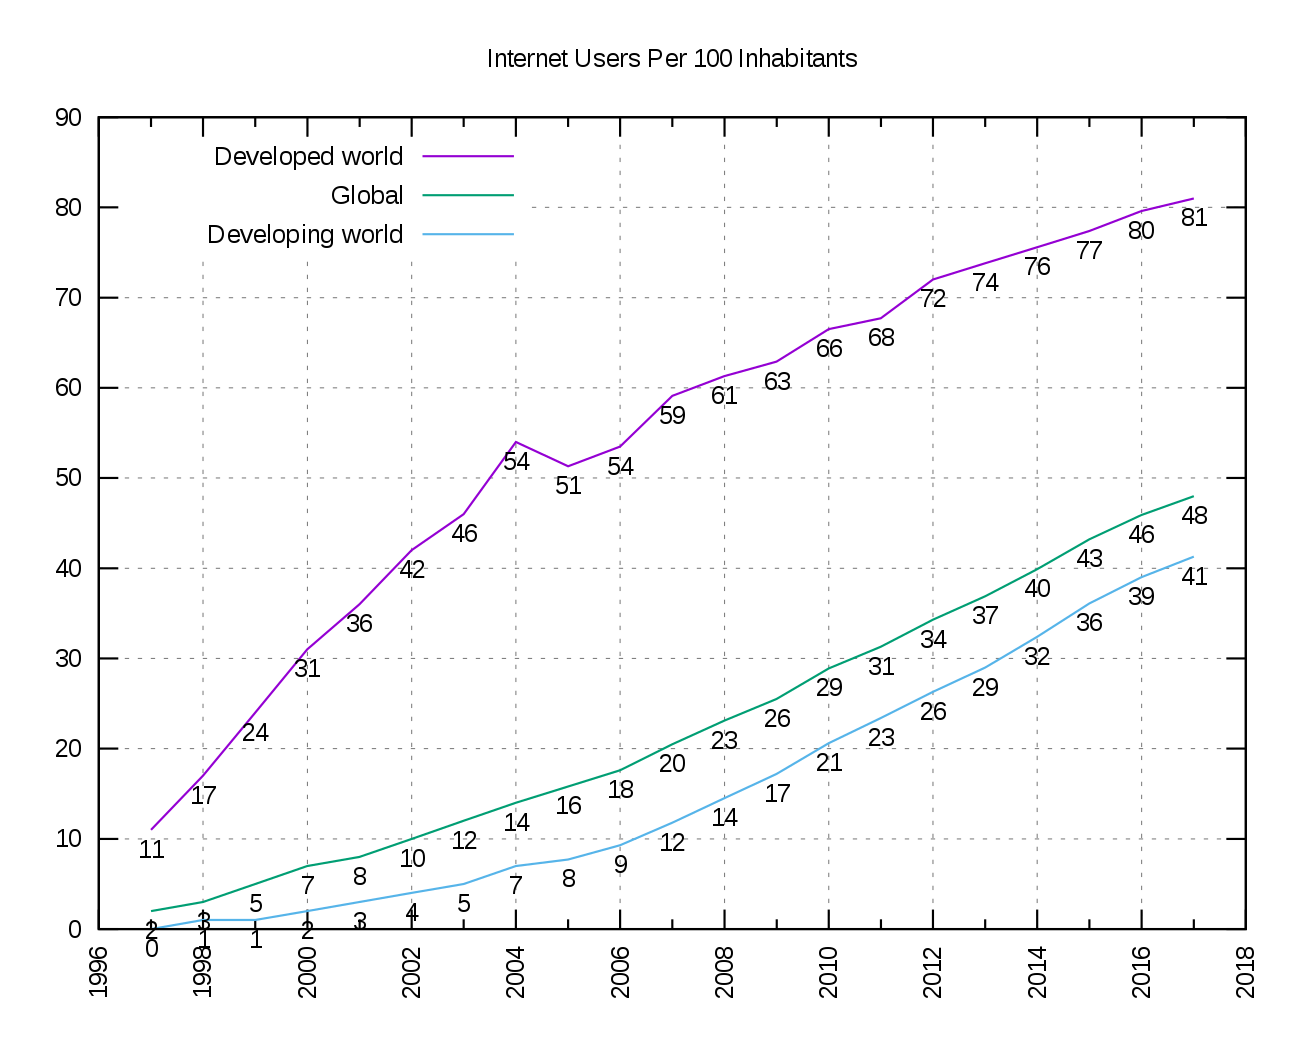
\includegraphics[scale=0.25]{internet_users}
    \caption{Porcentajes de uso de Internet - \textcopyright\ ITU \cite{internetusage}}
    \label{internetusageimagen}
\end{figure}

Con estos datos se pone en valor el hecho de que Internet es ya una parte indispensable en la vida de muchas personas, y que con el paso del tiempo aumentará mucho más su uso. Dicho esto, vamos a centrarnos en el ámbito universitario, desarrollando más este concepto de globalización y acotándolo al entorno de la universidad.\\\\

En la universidad de Granada se agrupan diferentes campus universitarios, repartidos en diferentes zonas del territorio de la capital, a saber:

\begin{itemize}
    \item Campus de Aynadamar
    \item Campus de Fuentenueva
    \item Campus Centro
    \item Campus de la Cartuja
    \item Campus de la Salud
\end{itemize}

Esta situación de separación entre los diferentes campus crea una serie de barreras o muros que en cierto modo limitan la interconexión entre ellos. Los profesores y alumnos de un campus pueden consultar en las diferentes páginas web institucionales, o visitar los edificios de otro campus, para poder conocer de primera mano lo que pasa en ellos, las actividades que se realizan, o cuáles son las líneas de investigación abiertas en algún departamento.\\

Pero la realidad es que, visitando las páginas web institucionales de las diferentes facultades y escuelas de la universidad, es dificil encontrar información al respecto. No todas se actualizan con regularidad, y no todas ofrecen los mismos contenidos, y por ello, no todas publican los proyectos o trabajos de investigaciónque están realizando.\\

Esta realidad que vivimos puede cambiar si hacemos un mejor uso del fenómeno de Internet y fomentamos más la interconexión entre distintos campus y facultades de la universidad, para así fomentar la cooperación y el trabajo en equipo.

\section{Motivación}
¿Qué motivación y razones nos llevan a comenzar un proyecto como éste? Existía un proyecto organizado por UGR Emprendedora \cite{ugremprende} como parte del programa Horizon 2020 \cite{h2020} que quería fomentar los equipos multidisciplinares.\\

En la actualidad los equipos de trabajo son muy frecuentes, y es habitual encontrar multitud de proyectos actualmente en desarrollo que son formados por muchas personas de diferentes ramas del conocimiento. Las capacidades y diferentes puntos de vista que aporta cada uno de los miembros se convierten en algo muy valioso que puede hacer que la idea o la investigación cobre más fuerza y solidez, a diferencia de desarrollarla sólo con el punto de vista de una única especialidad, que a menudo podría no contar con la misma profundidad.\\

En el ámbito universitario, el trabajo en equipo no es fomentado con demasiada frecuencia. Son diversos los factores que hacen poco atractiva la idea de cooperar en equipo con otras personas, siendo principalmente las siguientes:

\begin{itemize}
    \item A menudo no conoces al resto de tus compañeros.
    \item No conoces su grado de implicación y cooperación.
    \item No sabes si te dejarán a medias a mitad del trabajo.
\end{itemize}

Estos problemas se suman al hecho de que un trabajo en equipo requiere de un mayor esfuerzo de dedicación y entrega al mismo. En la etapa universitaria, a veces el exceso de trabajo de las asignaturas o la falta de motivación no son buenos aliados para fomentar proyectos multidisciplinares.\\

Con esta serie de problemas que se exponen, podemos hacernos una idea mental de la situación actual. La motivación por la que surge este proyecto es la de impulsar un cambio que haga darle la vuelta a la situación, encontrar las razones por las que actualmente fracasa el modelo de trabajo en equipo, y encontrar soluciones y formas de hacer ver su atractivo.\\

El hecho de querer mejorar la situación no es algo baladí. Poniendo como ejemplo práctico el caso de la Ingeniería Informática, en la actualidad todas las empresas del sector realizan su actividad con equipos de trabajo. En los últimos años está aumentando la adopción de metodologías de desarrollo ágil en el sector profesional, aunque este crecimiento es muy modesto todavía. \cite{agilereport}\\

La complejidad a la que han llegado hoy en día los sistemas y el software, hacen que sea necesario contar con varias personas que se encarguen de diferentes áreas del desarrollo. Además, la creciente inclusión de la informática y la tecnología en cada vez más sectores y ámbitos de la sociedad (sanidad, educación, trabajo social, etc) hacen que sea necesaria la cooperación y el entendimiento entre personas de otro campo profesional.\\

Esta tendencia sigue en aumento, pero no así la tendencia al trabajo en equipo en las universidades. Si conseguimos inclinar la balanza en favor de esta forma de trabajo, lograremos que las siguientes generaciones de graduados salgan más preparados para incorporarse a un equipo de trabajo y no tengan problemas para llevar a cabo su trabajo.\\

La demanda de equipos de trabajo multidisciplinares está aumentando, ya que se está comprobando la efectividad de los proyectos en los que intervienen profesionales de diferentes sectores y cada uno aporta sus habilidades al desarrollo en sí. Podemos ver ejemplos de ello en una serie de artículos que describen las mejoras en el ámbito sanitario aplicando equipos multidisciplinares (\cite{health1} y \cite{health2}). En la figura \ref{neuropedimagen} podemos ver la aplicación de este concepto en el Centro de Neurodesarrollo Pediátrico (NeuroPed).\\

\begin{figure}
    \centering
    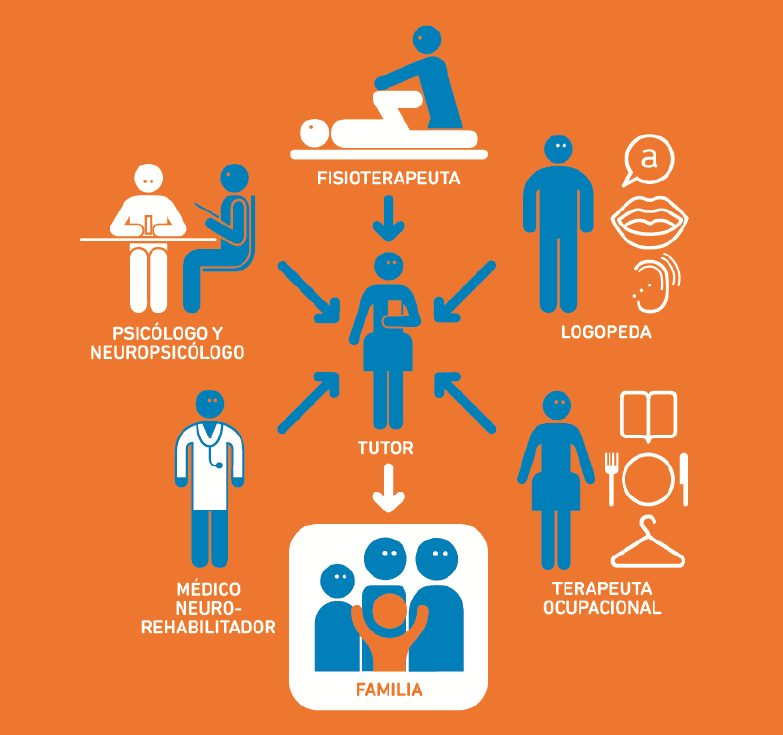
\includegraphics[scale=1.2]{neuroped}
    \caption{Equipo multidisciplinar - \textcopyright\ NeuroPed \cite{neuroped}}
    \label{neuropedimagen}
\end{figure}

Pero no todo se basa en el concepto de \textit{fomentar los proyectos en equipo}, con esto se pretende también dar respuesta a la necesidad y deseo de algunas personas de que los proyectos en equipo sean algo más habitual durante su etapa en la universidad. La distanciación entre campus complica el que un o una estudiante se interese por saber lo que pasa en otros campus. Además, algunos estudiantes cuentan con ideas muy interesantes que les gustaría poder llevar a cabo, y en algunas de ellas necesitan contar con gente que sepa de otras ramas del conocimiento.\\

En la motivación de este proyecto se encuentra también el lograr que dichos estudiantes puedan hacer pública su idea y que llegue al máximo número de personas del sector universitario, otros estudiantes de diferentes disciplinas que quieran unirse a dicha idea y aportar su punto de vista.\\

En definitiva, este proyecto surge con la motivación de romper barreras, facilitar los proyectos en equipo y fomentar sus diversas ventajas. En el siguiente capítulo se hablarán de los objetivos planteados para este trabajo, y se hablará un poco del estado del arte de diversos aspectos a considerar para el mismo.

\section{Estructura de este documento}
Este primer capítulo ha querido servir como introducción al contexto que desarrolla este trabajo y la motivación por la que ha surgido. A continuación se detallan, de forma resumida, los contenidos del resto de capítulos de este documento:

\begin{itemize}
    \item En el \textit{capítulo \ref{ch:objetivos}} (\textbf{Objetivos}), se describen los diferentes objetivos que se han definido inicialmente para este trabajo, así como un breve estado del arte sobre ciertos aspectos relacionados con el proyecto.
    \item En el \textit{capítulo \ref{ch:metodologia}} (\textbf{Metodología}), se detallan las diferentes tareas y procedimientos que se pueden utilizar para llevar a cabo la gestión de un equipo multidisciplinar. También se encuentra desarrollado en este capítulo cuáles han sido los diferentes integrantes del equipo, y cuáles son las tareas que inicialmente realizará cada uno de ellos.
    \item En el \textit{capítulo \ref{ch:desarrollo}} (\textbf{Desarrollo}), se abarca del trabajo realizado por mí, el desarrollo del producto, es decir, la aplicación web de SmartU para la publicación de proyectos y difusión de opiniones e ideas. Se estructura en diversos apartados siguiendo la estructura típica del proceso de desarrollo de software. Se muestra la aplicación web creada, describiendo sus características y su interfaz de usuario.
    \item En el \textit{capítulo \ref{ch:conclusiones}} (\textbf{Resultados y Conclusiones}), se recopilan tanto lo que se ha hecho a lo largo del desarrollo de este trabajo como las conclusiones y resultados finales obtenidos de esta experiencia. Se comentan además una serie de mejoras para el futuro que se podrían aplicar.
    \item En el \textit{capítulo \ref{ch:anexos}} (\textbf{Anexos}), se incluyen materiales adicionales que complementan la información de algunos de los capítulos de esta documentación.
\end{itemize}
